\documentclass[12pt,twoside]{scrreprt}
\usepackage[T1]{fontenc}
\usepackage[utf8]{inputenc}
\usepackage{lmodern}
\usepackage{textcomp}
\usepackage[francais]{babel, varioref}
\usepackage{graphicx}
\usepackage{listings}
\usepackage{xspace}
\usepackage{amsmath}
\usepackage{amssymb}
\usepackage{calc}
\usepackage{listingsutf8}
\usepackage{color}
\usepackage{xcolor}
\usepackage{afterpage}
\usepackage[style=verbose-note,backend=bibtex]{biblatex}
\usepackage{url}
\usepackage[top=2.1cm,bottom=2.2cm,left=2cm,right=2cm]{geometry}
\usepackage[final]{pdfpages}
\usepackage{subcaption}
\usepackage{amsmath}
\usepackage{array}
\captionsetup{compatibility=false}

\lstdefinelanguage{xml}{morestring=[b]",
                        morestring=[s]{>}{<},
                        morecomment=[s]{<?}{?>},
                        stringstyle=\color{black},
                        identifierstyle=\color{black},
                        keywordstyle=\color{cyan},
                        morekeywords={ROOT,S,NP,VP,ADVP,PRP\$,NN,NNP,NNS,JJ,DT,VBD,PP,PDT,TO,IN}% list your attributes here
                        }


\lstset{language=xml,
        escapeinside={K}{W},
        %basicstyle=\ttfamily,
        columns=fullflexible,
        commentstyle=\color{gray}\upshape
        tabsize=3,
        label=code:sample,
        frame=shadowbox,
        rulesepcolor=\color{gray},
        xleftmargin=20pt,
        framexleftmargin=15pt,
        numbers=left,
        numberstyle=\tiny,
        numbersep=5pt,
        breaklines=true,
        showstringspaces=false,
        basicstyle=\footnotesize,
        emph={food,name,price},emphstyle={\color{magenta}}
        }

\newcommand{\hlc}[2][yellow]{ {\sethlcolor{#1} \hl{#2}} }
\newcommand{\highlight}[2][yellow]{\mathchoice%
  {\colorbox{#1}{$\displaystyle#2$}}%
  {\colorbox{#1}{$\textstyle#2$}}%
  {\colorbox{#1}{$\scriptstyle#2$}}%
  {\colorbox{#1}{$\scriptscriptstyle#2$}}}

\definecolor{gray}{rgb}{0.4,0.4,0.4}
\definecolor{darkblue}{rgb}{0.0,0.0,0.6}
\definecolor{cyan}{rgb}{0.0,0.6,0.6}

% Pour sommaire cliquable
\usepackage{hyperref} % Créer des liens et des signets
\hypersetup{
colorlinks=true, %colorise les liens
breaklinks=true, %permet le retour à la ligne dans les liens trop longs
urlcolor= blue, %couleur des hyperliens
linkcolor= black, %couleur des liens internes
citecolor=black,  %couleur des références
}

% Fichier de bibliographie
\bibliography{parties/biblio}

\usepackage{templateINSA}
\initINSA

% Tirte centre
\renewcommand\infoBig{Baptiste O'Jeanson}
\renewcommand\infoSmall{Rapport de stage de spécialité}

% Titre bas
\title{Classification de signaux entreprises avec une approche machine learning}
\renewcommand\soustitre{Information retrieval, Text mining and Natural Language Processing}

% Auteurs
\author{
	\textbf{Étudiant:} Baptiste \bsc{O'Jeanson} \\
	\textbf{Maître de stage:} Christian \bsc{Frisch}\\
	\textbf{Entreprise:} Data Publica\\
	\textbf{Année:} 2014-2015\\
	\textbf{Dates:} du 01/06/2015 au 28/08/2015\\
	\textbf{Lieu:} Paris, France\\
	}

\begin{document}

% titleINSA : Page de garde
% #1 : descendre le titre du milieu (en mm)
% #2 : lien de l'image de fond
% #3 : décalage sur X de l'image de fond (en mm)
% #4 : décalage sur Y de l'image de fond (en mm)
% #5 : largeur de l'image de fond de #5 (en mm)
% #6 : Crédit de l'image de fond
 \titleINSA{0}{images/logo-data-publica.jpg}{0}{50}{220}{Image : \href{http://www.data-publica.com/}{\color{white}{http://www.data-publica.com/}}}


% Remerciements
\section*{ \begin{center} \textbf{ {\LARGE Remerciements} } \end{center} }
\phantomsection

Premièrement, j'aimerais remercier François Bancilhon \footnote{Francois Bancilhon, présenté ici \ref{fig:teamc_data_publica}}, directeur général de Data Publica, et Christian Frisch \footnote{Christian Frisch, présenté ici \ref{fig:teamd_data_publica}}, directeur technique de Data Publica, de m'avoir donné l'opportunité de découvrir le monde du travail en start-up. Je voudrais aussi les remercier de m'avoir fait confiance et de m'avoir confié une mission très intéressante.

\paragraph{}
Ensuite, je voudrais remercier Samuel Charron, Clément Chastagnol et Guillaume Lebourgeois qui m'ont encadré, suivi et conseillé durant mon stage, et qui ont enrichi mes connaissances du monde professionnel ainsi que mes connaissances en informatiques.

\paragraph{}
J'aimerais aussi remercier tout particulièrement Thomas Dudouet, qui a fait suite à ma candidature spontanée, et qui m'a donc offert cette chance de pouvoir m'entretenir avec Clément Chastagnol puis Christian Frisch.

\paragraph{}
Je souhaiterais également remercier l'ensemble de l'équipe de développeurs et l'ensemble de l'équipe de marketing de m'avoir accueilli si chaleureusement.

\paragraph{}
Enfin, merci à mon tuteur de stage, Nicolas Malandain, pour sa disponibilité.
\addcontentsline{toc}{chapter}{Remerciements}

% Sommaire
\tableofcontents

% Parties
\chapter{Présentation de l'entreprise}
L’évolution des technologies et leurs usages ont fait exploser la quantité de données générées. Selon IBM, 2.5 milliard de gigabytes (GB) de données a été générée tout les jours de l'année 2012. De plus, cette quantité de données, double tout les deux ans. Cependant, seules 0,05\% de ces données sont analysées.\\

L’exploration ou la fouille de données (\og data mining \fg) consiste à en extraire des informations utiles, et ceci peut s’avérer très fructueux. La question principale qui se pose est de savoir comment utiliser intelligemment cette immense masse de données pour en tirer une plus-value ?\\
C’est le rôle des entreprises spécialisées dans l'exploitation de ces données.

\section{L'entreprise}
    La société Data Publica a été fondée en juillet 2011 par François Bancilhon et Christian Frisch, respectivement l'actuel directeur général et l'actuel directeur technique.

    \subsection{L'activité de Data Publica}
        Data Publica est un des précurseurs de l'open data en France. \textcolor{red}{Cette société , qui a bénéficiée d’investissements technologiques faits en 2010 dans le cadre d’un projet de R\&D, a été financée initialement par un groupe de business angels et le fonds d’amorçage \textbf{IT Translation}.}
        Data Publica est un start-up spécialisée dans les données entreprises, l'open data, le big data et la dataviz. C'est une société relativement jeune, axée R\&D. Son leitmotiv, alimenté par une équipe très dynamique et compétente, est la recherche constante du dépassement technique.

        \paragraph{}
            Historiquement, Data Publica ne faisait que de l'open-data. C'est-à-dire que la société se servait de données accessibles à tous (provenant d'institutions gouvernementales notamment) pour créer des jeux de données sur mesure pour des entreprises. Ainsi, la société s'est spécialisé dans l'identification des sources de données, leur extraction et leur transformation en données structurées.

        \paragraph{}
            Depuis quelques années, Data Publica se spécialise dans les données sur les entreprises française en dépit de son activité open-data qu'elle a progressivement mis de côté. Les services qu'elle propose ne sont plus tout-à-fait les mêmes. En effet, Data Publica réutilise les données open-data concernant les entreprises française dans son produit phare. Ce produit est lui même conçu pour les entreprises du B2B. Le produit est décrit en partie \ref{c_radar}.

        \paragraph{}
            Data Publica participe également à de nombreux projets de recherche français et européens tels que XDATA, Diachron ou Poqemon, en partenariat avec l'INRIA.

    \subsection{L'équipe de Data Publica}
        Data Publica emploie 14 personnes réparties en 2 équipes : une équipe commerciale (4 personnes) et une équipe technique (10 développeurs). Les deux équipes travaillent chacune dans son open-space. Pendant mon stage, j'ai été immergé au sein de l'équipe technique.

        \paragraph{L'équipe technique :}
            Elle est composé de 10 développeurs (ordonnés par ancienneté visible en figure \ref{fig:teamd_data_publica}) :
            \begin{itemize}
                \item Christian Frisch, directeur de l'équipe
                \item Thomas Dudouet, \textcolor{red}{Java / Back end développeur}
                \item Guillaume Lebourgeois, chef de produit C-Radar
                \item Samuel Charron, \textcolor{red}{Data scientist Python et mon maître de stage}
                \item Loïc Petit, \textcolor{red}{Java JBM}
                \item Clément Chastagnol, \textcolor{red}{data scientist Python et mon maître de stage}
                \item Clément Déon, \textcolor{red}{Front end développeur}
                \item Fabien Bréant, \textcolor{red}{Back end développeur}
                \item Jacques Belissent, \textcolor{red}{?}
                \item Vincent Ysmal, \textcolor{red}{Java / Back end développeur}
            \end{itemize}

        \begin{figure}[h!]
            \centering
            \begin{subfigure}[b]{0.2\textwidth}
                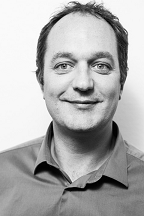
\includegraphics[width=\textwidth]{images/christian-serieux.png}
                \caption{Christian F.}
                \label{fig:christian}
            \end{subfigure}
            \begin{subfigure}[b]{0.2\textwidth}
                
\includegraphics[width=\textwidth]{images/thomas2-Copier-Copier.jpg}
                \caption{Thomas D.}
            \end{subfigure}
            \begin{subfigure}[b]{0.2\textwidth}
                
\includegraphics[width=\textwidth]{images/guillaume-serieux.png}
                \caption{Guillaume L.}
            \end{subfigure}
            \begin{subfigure}[b]{0.2\textwidth}
                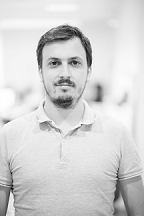
\includegraphics[width=\textwidth]{images/samuel-serieux.png}
                \caption{Samuel C.}
            \end{subfigure}
            \begin{subfigure}[b]{0.2\textwidth}
                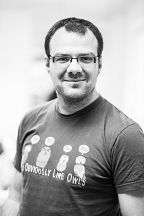
\includegraphics[width=\textwidth]{images/loic-serieux.png}
                \caption{Loïc P.}
            \end{subfigure}
            \begin{subfigure}[b]{0.2\textwidth}
                
\includegraphics[width=\textwidth]{images/clement-c-serieux.png}
                \caption{Clément C.}
            \end{subfigure}
            \begin{subfigure}[b]{0.2\textwidth}
                
\includegraphics[width=\textwidth]{images/clement-d-serieux.png}
                \caption{Clément D.}
            \end{subfigure}
            %\begin{subfigure}[b]{0.2\textwidth}
            %    
\includegraphics[width=\textwidth]{images/jacques.jpg}
            %            \caption{Jacques B.}
            %\end{subfigure}
            \begin{subfigure}[b]{0.2\textwidth}
                
\includegraphics[width=\textwidth]{images/vincent.jpg}
                \caption{Vincent Y.}
            \end{subfigure}
            \caption{L'équipe technique de Data Publica}
            \label{fig:teamd_data_publica}
        \end{figure}

\newpage

        \paragraph{L'équipe commerciale :}
            Elle est composé de 4 commerciaux (ordonnés par ancienneté visible en figure \ref{fig:teamc_data_publica}) :
            \begin{itemize}
                \item François Bancilhon, directeur général
                \item Benjamin Gans, Responsable Communication et Marketing
                \item Emmanuel Jouanne, Business Development Manager
                \item Philippe Spenato, Ingénieur d'affaire
                \item Justine Pourrat, Responsable Communication et marketing
            \end{itemize}

        \begin{figure}[h!]
            \centering
            \begin{subfigure}[b]{0.2\textwidth}
                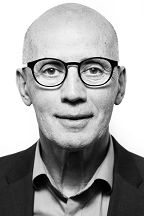
\includegraphics[width=\textwidth]{images/francois-serieux.png}
                \caption{François B.}
                \label{fig:francois}
            \end{subfigure}
            \begin{subfigure}[b]{0.2\textwidth}
                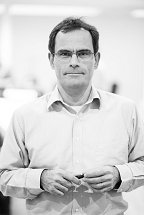
\includegraphics[width=\textwidth]{images/philippe-1-serieux.png}
                \caption{Philippe S.}
            \end{subfigure}
            \begin{subfigure}[b]{0.2\textwidth}
                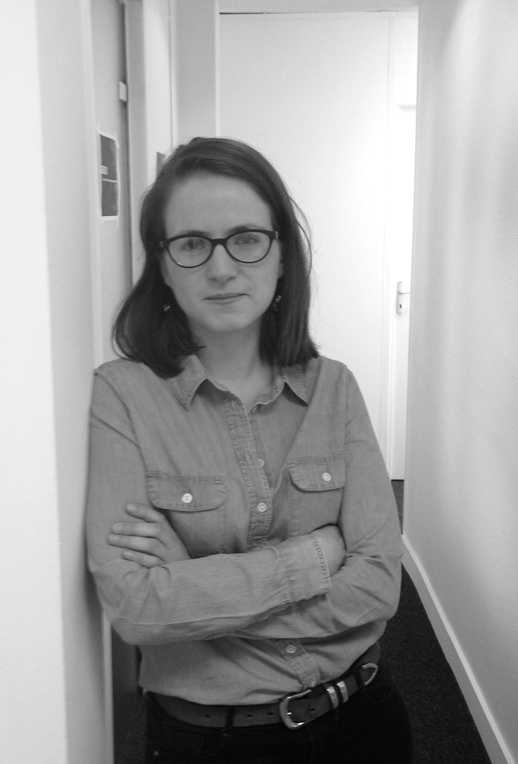
\includegraphics[width=\textwidth]{images/Justine-serieuse-crop.jpg}
                \caption{Justine P.}
            \end{subfigure}
            \caption{L'équipe commerciale de Data Publica}
            \label{fig:teamc_data_publica}
        \end{figure}

\section{C-Radar}\label{c_radar}
    \subsection{Présentation commerciale de C-Radar}
        Son produit est un moteur de recherche B2B (Business to Business). Celui-ci a pour objectif de permettre aux services ventes et marketing des entreprises B2B de vendre plus et mieux.\\
        Ce moteur de recherche, appelé C-Radar, est un produit de vente prédictive construit sur une base de référence des entreprises françaises. Il regroupe beaucoup d'informations sur les entreprises françaises, dont notamment leurs informations administratives, financières et toutes celles qui découlent de leur communication sur les réseaux sociaux et le web.\\

        C-Radar est un concentré de technologies du big data. En effet, il utilise diverses technologies comme le crawling, le scraping ou encore le machine learning. Ceci afin d'offrir à l'utilisateur diverses fonctionnalités : moteur de recherche d'entreprises, fiche d'activité d'entreprises avec contacts commerciaux, détection de nouveaux prospects, scoring de prospects existants, segmentation automatique d'entreprises, identification de marché, etc.

    \subsection{Présentation technique de C-Radar}
        \subsubsection{Les technologies utilisées par C-Radar}
            Pour répondre aux problématiques auxquelles Data Publica se confronte, la société a acquis 4 expertises majeures :
            \begin{itemize}
                \item Le web crawling / web scraping : la récupération des données ;
                \item Le data mining / text mining : l'analyse, l’extraction et l’enrichissement des données;
                \item Le machine learning : l'apprentissage automatique à partir de données structurées ;
                \item La dataviz : la visualisation des données.
            \end{itemize}

            \paragraph{Le crawling :}
                Le crawling est l’action réalisée par un programme informatique, appelé le web crawler, qui va de site en site afin d’en extraire automatiquement toute l’information qui est présente sur les différentes pages. Cette technique est utilisée notamment pour l’extraction de données non structurées: la structure du site n’est pas connue à l’avance, l’extraction des données se fait directement sur le contenu (c’est à dire le code HTML) de la page crawlée. Ce processus est \og brutal \fg.

            \paragraph{Le scraping :}
                Le scraping est l’action réalisée par un programme informatique pour extraire des unités d’information structurées d’un site web. Contrairement au crawling, il est question d’extraire des données précises, et pas la totalité des données disponibles sur le site. Le site “scrappé” et sa structure doivent donc être connus et analysés à l’avance afin d’adapter le scraper au site. Ce processus est \og intelligent \fg.

            \color{red}

            \paragraph{Le data mining / text mining :}
                Une fois des sites web crawlés et scrapés, ou que des flux (RSS ou réseaux sociaux) aient été captés, on peut commencer à analyser le contenu récupéré à la recherche d'informations sous forme de patterns particuliers, par exemple. On analyse afin de normaliser des problèmes d'encodages, de structures de date, de numéros de téléphone, etc.\\
                Globalement, cette phase consiste à regarder les données \og dans le fonds des yeux \fg \autocite{steph_canu} afin de voir leurs fonds mais aussi leurs formes.

            \paragraph{Le machine learning :}
                Quand les données sont correctement formatées et normalisées, on peut construire des applications capable d'apprendre automatiquement de ces données, de les classifier. Ainsi quand on aura une nouvelle donnée l'application sera capable de prédire sa classe d'après ses caractéristiques.\\
                L'idée derrière le machine learning est de pouvoir extraire automatiquement des informations d'une nouvelle donnée et ainsi prédire une classe de donnée.

            \paragraph{La dataviz :}
                C'est la dernière étape. Elle présente les données de manière visuelle et interprétable. Ainsi, on peut comprendre plus facilement et rapidement les informations extraites des données.


        \subsubsection{L'architecture technique de C-Radar}
            L'architecture de C-Radar peut être divisée en plusieurs parties (visible en figure \ref{fig:archi}) :
            \begin{itemize}
                \item Différentes bases de données pour différents stockages (une base de données Mongo, une base de données Cassandra et une base de données PostGreSQL) ;
                \item Un moteur de recherche sémantique (Elastic Search) ;
                \item Un gestionnaire de queue (RabbitMQ) ;
                \item Différents plugins Python s'interfaçant avec le gestionnaire de queue RabbitMQ ;
                \item Un gestionnaire de flux entre les différents composants précédents, le Workflow ;
                \item Une application Java s'interfaçant avec Elastic Search et les bases de données Mongo et PostGreSQL.
            \end{itemize}

            \paragraph{Le JBM ou Java Base Manager :}
                Le JBM est le projet Java qui rassemble le Workflow et l'application \href{app.c-radar.com}{app.c-radar.com}. Ce projet a été conçu et construit au dessus de Spring. Spring est un framework Java permettant de créer des applications web. Il prend en charge énormément de chose dont notamment le modèle MVC, la sécurité de l'application, l'interface avec les gestionnaire de queue, etc. (Pour plus d'information, voir \href{http://spring.io/}{http://spring.io/}).

            \paragraph{Le Workflow :}
                Le Workflow est le gestionnaire de flux permettant de lancer les différents processus de récupération et d'analyses des données. Il gère tout ce qui est \og computing \fg. Par exemple, c'est lui qui lance RabbitMQ qui lui même lance l'exécution des plugins Python gérant le processus de crawling de sites web, par exemple. Une fois les sites webs crawlés, le Workflow va les stocker dans Cassandra. Il gère tout ce qui est exécution des plugins Python (crawling et scraping du web, capture et catégorisation des signaux, etc), stockage des données produites à l'issue de ces exécutions et indexation dans Elastic Search.\\
                Pour résumer, il prépare les données que l'application va se charger de présenter à l'utilisateur.

            \paragraph{L'application \href{app.c-radar.com}{app.c-radar.com} :}
                L'application, \og présente \fg les données aux utilisateurs. Elle fait le reporting des données produites par le Workflow. Elle permet de rechercher des entreprises, de voir leur répartitions géographiques, de créer des listes d'entreprises, etc. C'est l'application visible et utilisée par l'utilisateur.

            \paragraph{Les bases de données :}
                Les bases de données stockent différentes données. La base Mongo stocke les données liées aux entreprises et les signaux, par exemple.

            \paragraph{Les plugins Python :}
                Enfin, les plugins Python sont des applications Python connectées à d'autres composants, afin d'exécuter une tâche sur des données. Ces données sont reçues des autres composants et le plugin leur retourne les résultats de sa tâche.

            \color{black}


            \begin{figure}[h!]
                \centering
                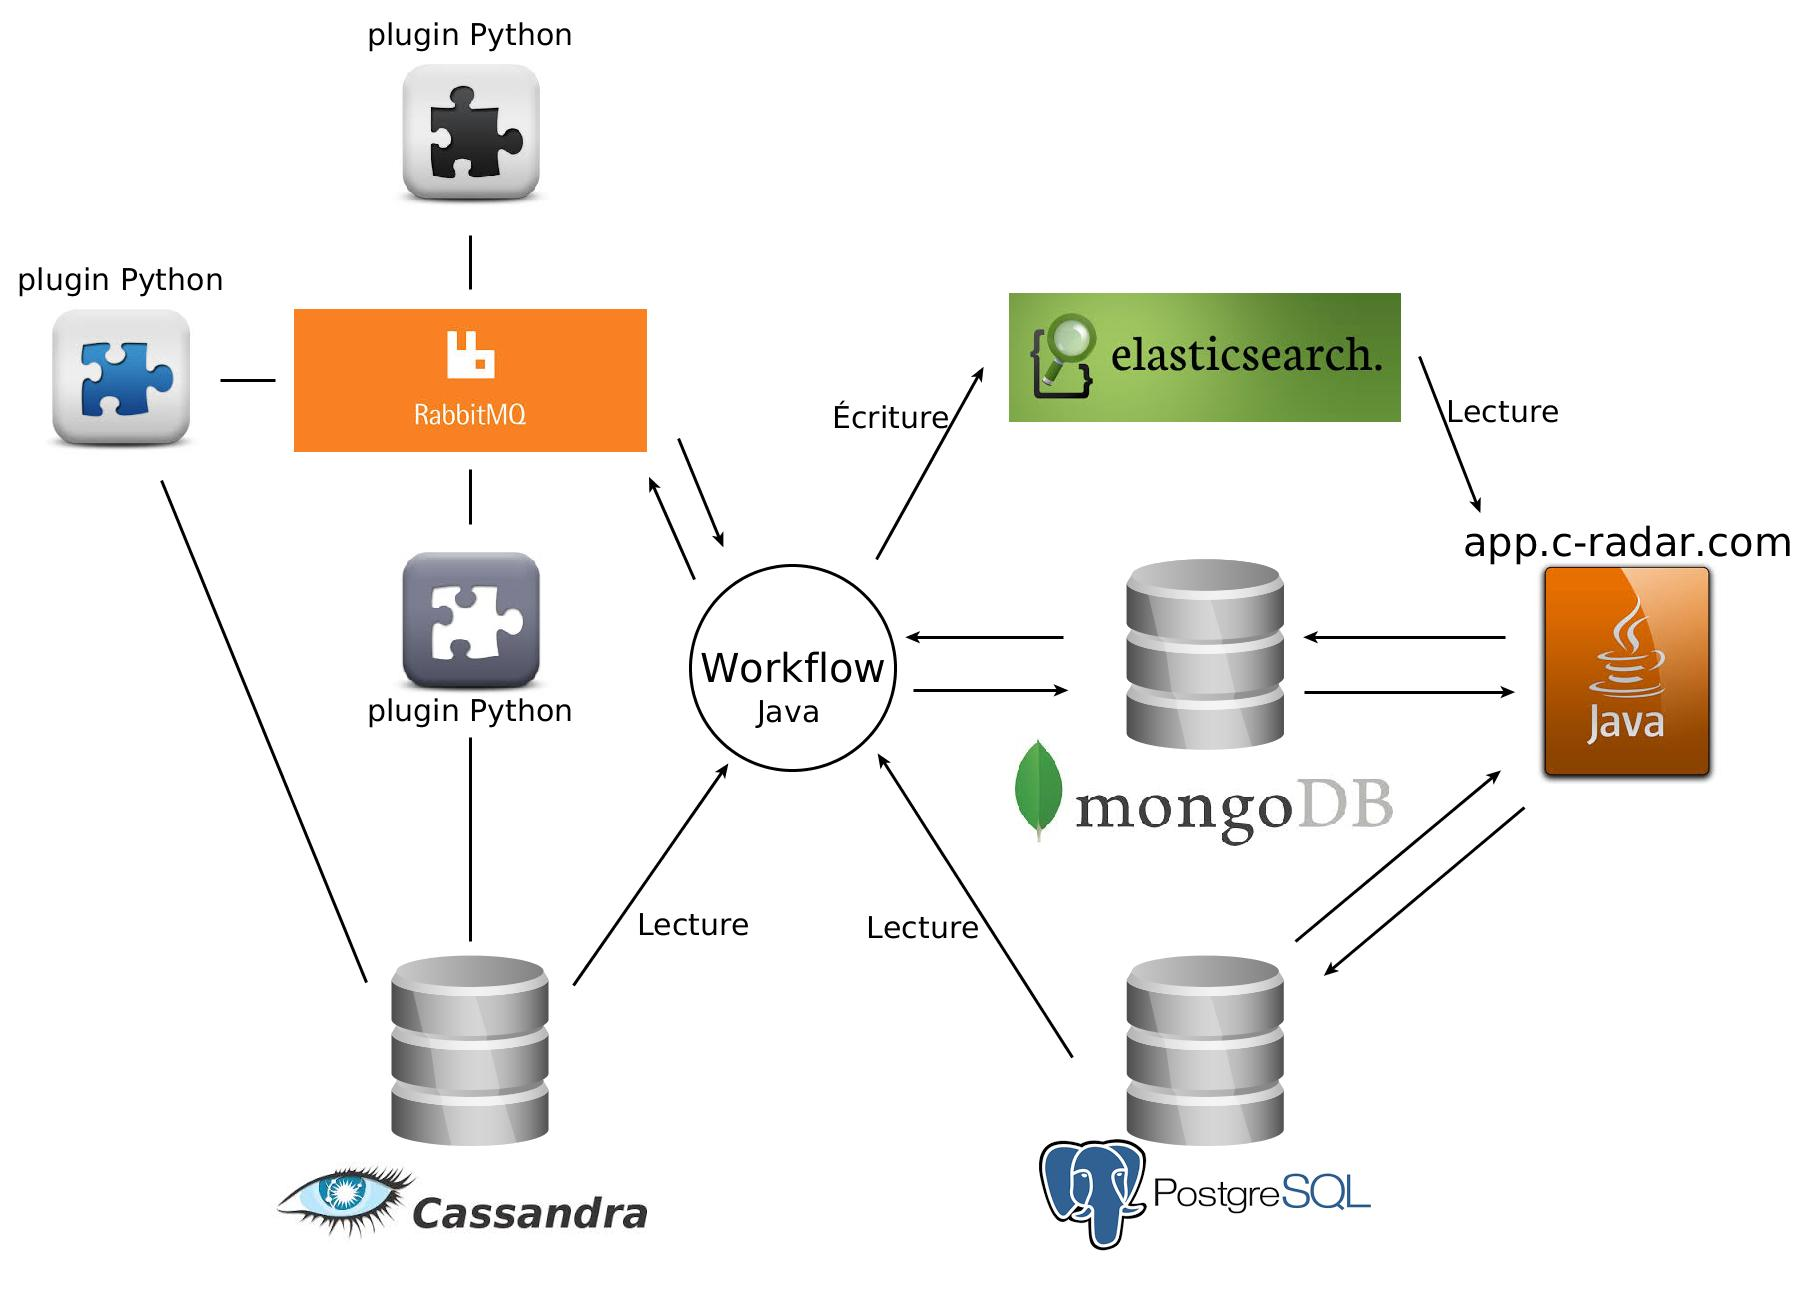
\includegraphics[width=\textwidth]{images/archi.jpg}
                \caption{L'architecture générale de C-Radar}
                \label{fig:archi}
            \end{figure}

\chapter{Présentation du sujet}
À la suite d'une candidature spontanée et de premiers contacts avec Thomas Dudouet et Clément Chastagnol, je me suis entretenu avec Christian Frisch afin de savoir quelle pourrait être ma contribution chez Data Publica. Ayant suivi une formation à l'INSA plutôt orienté big data / data mining, Christian Frisch m'a alors proposé de travailler sur l'une des fonctionnalités du produit C-Radar.

\section{La fonctionnalité de C-Radar} % (fold)
\label{sec:la_fonctionnalite_de_c_radar}
    L'objectif de mon stage serait le suivant : améliorer la fonctionnalité de C-Radar permettant d'être au courant de l'intégralité de la communication des entreprises françaises et belges simplement en s'abonnant à une newsletter.\\

    \begin{figure}[h!]
        \centering
        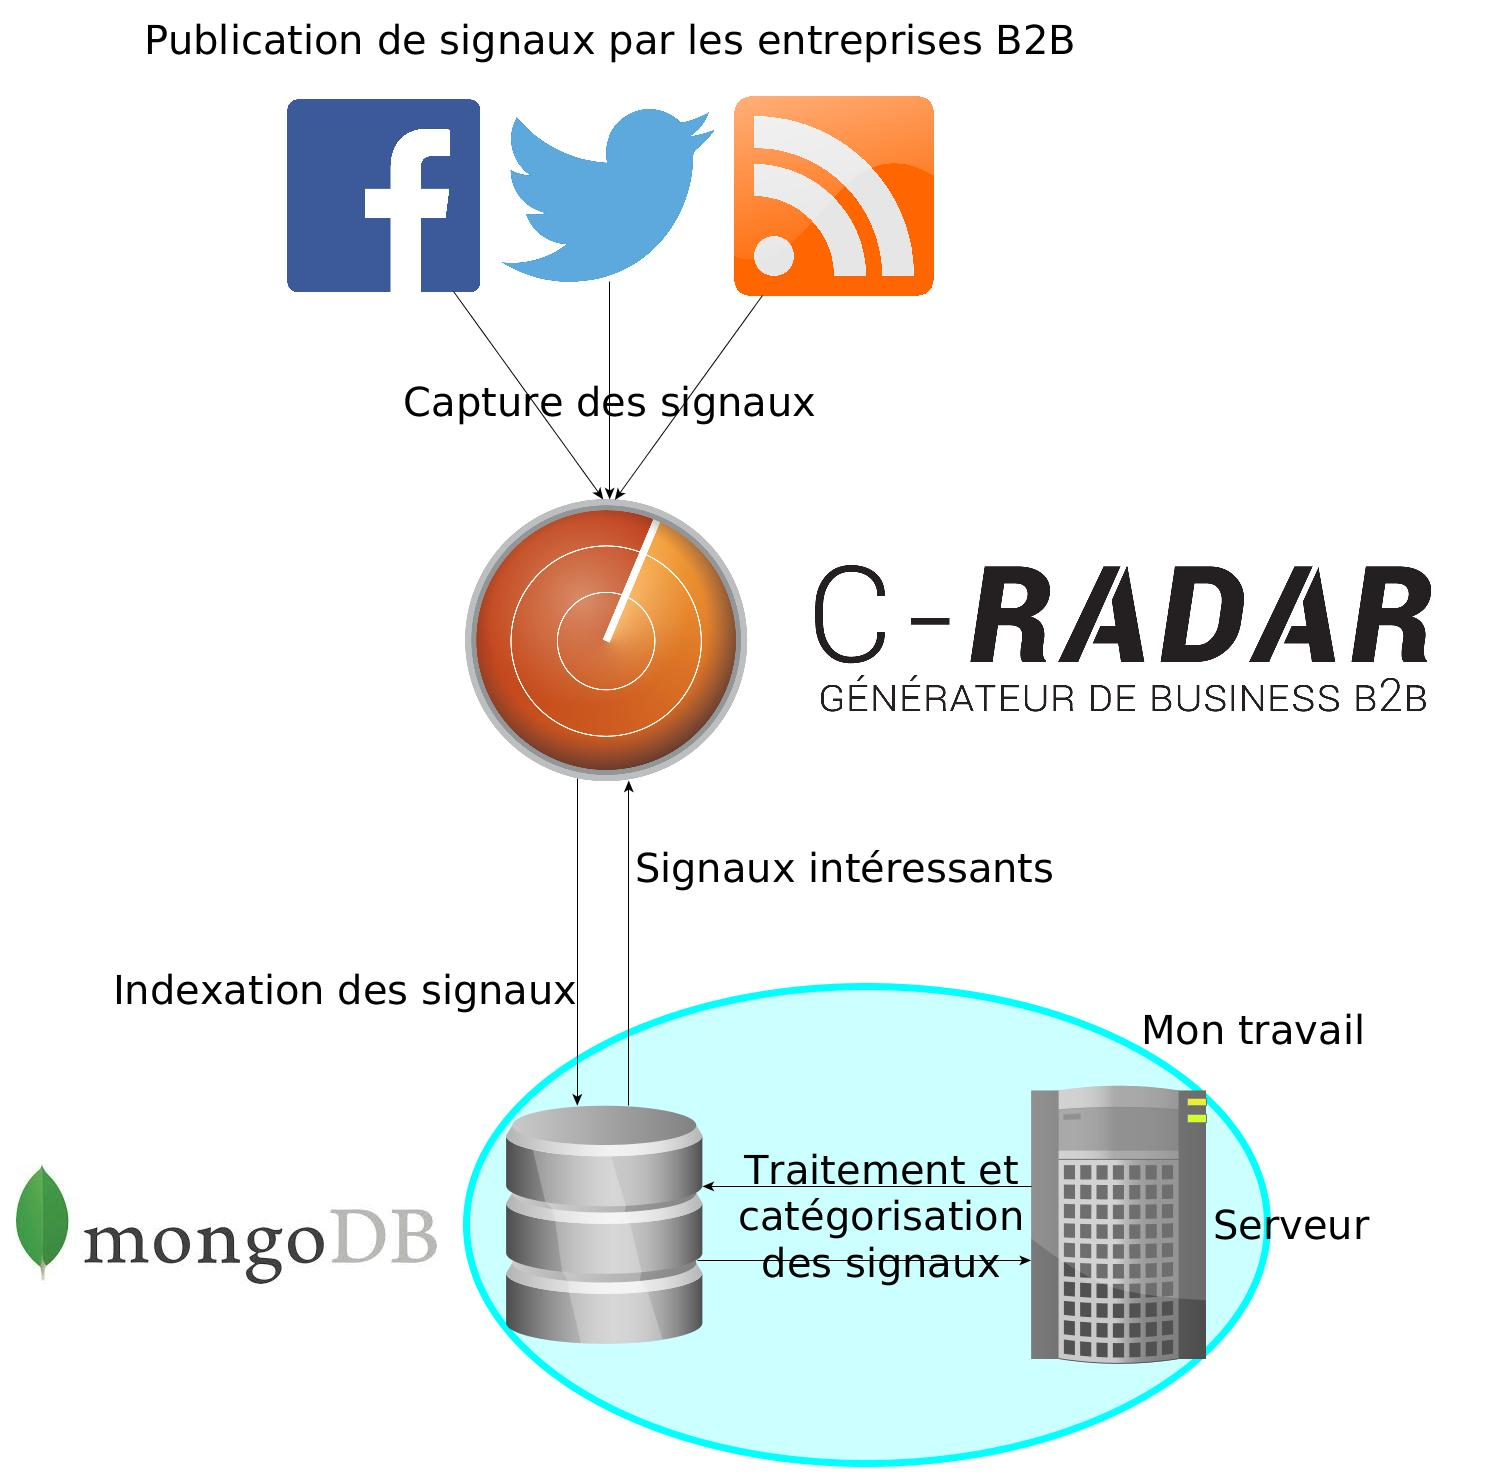
\includegraphics[width=0.75\textwidth]{images/capture_process.jpg}
        \caption{Le fonctionnement général de cette fonctionnalité.}
        \label{fig:capture_process}
    \end{figure}

    De l'offre d'emploi, à la participation à des salons, en passant par les nominations de personnel ainsi que les présentations des derniers produits ou encore des éventuelles levées de fonds ou investissements, la communication des entreprises n'est plus équivoque mais bel et bien ordonnée grâce à cette fonctionnalité. On peut désormais savoir quels sont les derniers postes à pourvoir chez Orange, par exemple, ou encore les dernières nominations qui ont eu lieux à la Banque Postale.\\

    Le fonctionnement général de cette fonctionnalité est le suivant (visible en figure \ref{fig:capture_process}) :
    \begin{enumerate}
        \item C-Radar capte tous les signaux émis par les entreprises sur les réseaux sociaux (Facebook et Twitter), dans les médias ou via des flux RSS. Ces signaux sont ensuite stockés dans une base de données Mongo.
        \item Une fois ces signaux capturés et stockés, il faut les traiter afin d'identifier l'intérêt potentiel de leur contenu.
    \end{enumerate}
    C'est sur ce second point que j'interviens.
% section la_fonctionnalit_de_c_radar (end)

\section{Ma mission chez Data Publica} % (fold)
\label{sec:ma_mission_chez_data_publica}
    Ma mission est de construire une chaîne de traitement automatique, un plugin Python, récupérant la liste des signaux émis par les entreprises en entrée depuis un point d'API, leur appliquer les traitements nécessaires afin de fournir, en sortie, la liste des signaux intéressants ainsi que leur catégorie respective.\\

    Il s'agit donc de construire une application, un plugin Python, capable de classifier un signal dans une catégorie par la seule connaissance de son contenu (éventuellement un titre). L'application traitera donc des documents textuels.\\
    Le travail se divise en deux étapes :
    \begin{enumerate}
        \item Appliquer une série de prétraitements sur le contenu des signaux afin de sélectionner les features jugés porteurs d'information. En effet, comme les données manipulées sont textuelles, il faut filtrer certaines chaînes de caractères considérées comme du bruit.
        \item Construire un classifieur à partir des features sélectionnés parmi les données que l'on juge porteuses d'information.
    \end{enumerate}

    \subsection{Inscription dans le domaine du \textit{Big Data}}
        Les tâches qui découlent de ma mission, et notamment tous les prétraitements, sont directement liées à la discipline de la fouille de textes (\textit{Text Mining}) (et de l'\textit{Information Retrieval}) pour trouver des informations dans le contenu des signaux. Elles sont également liées à la discipline du traitement automatique du langage naturel (\textit{Natural Language Processing}). Enfin, la construction du classifieur automatique implique des compétences en \textit{Machine Learning}.

        \paragraph{Remarque :}
            Un classifier est un outils d'apprentissage automatique qui prend des données et les classifie dans k classes.

    \subsection{Synthèse du travail à réaliser}
        Si l'on devait résumer le travail à effectuer (visible en figure \ref{fig:capture_process}), on pourrait le synthétiser comme ceci : Construire une application (plugin Python), qui prend en entrée un signal émis par une entreprise et répond aux questions suivantes :
        \begin{enumerate}
            \item Ce signal a-t-il de l'intérêt ?
            \item Si oui, quel est le sujet du signal ? Parle -t-il d'une offre d'emploi, d'une nomination, d'une levée de fond, etc ?
        \end{enumerate}
        La figure \ref{fig:process} montre ce que l'application (le plugin Python) doit être capable de faire.

        \begin{figure}[h!]
            \centering
            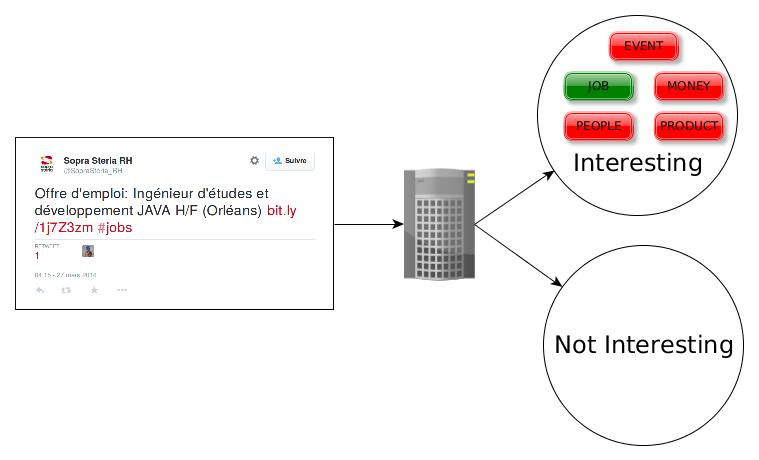
\includegraphics[width=\textwidth]{images/process.jpg}
            \caption{La tâche du plugin Python.}
            \label{fig:process}
        \end{figure}

\section{Présentation des signaux}
\label{sec:etat_bd}
    Les signaux sont des posts Facebook, des tweets ou bien des flux RSS publiés par des entreprises.

    \paragraph{Hypothèses de départ :}
        On considérera qu'un signal est intéressant si son contenu a pour sujet :
        \begin{itemize}
            \item Une offre d'emploi (ou un stage) à pourvoir au sein de l'entreprise qui l'a postée. Par la suite, on associera le tag \textit{JOB} à cette catégorie.
            \item Un évènement auquel l'entreprise participe (un salon par exemple). Par la suite, on associera le tag \textit{EVENT} à cette catégorie.
            \item Un produit que l'entreprise vient de présenter. Par la suite, on associera le tag \textit{PRODUCT} à cette catégorie.
            \item Une nomination d'un employé dans l'entreprise ou d'une entreprise vers une autre entreprise. Par la suite, on associera le tag \textit{PEOPLE} à cette catégorie.
            \item Une levée de fonds, un investissement, ou encore une déclaration de résultats ou de chiffre d'affaire.. Par la suite, on associera le tag \textit{MONEY} à cette catégorie.
        \end{itemize}

    \paragraph{Exemple de signal type pour chaque catégorie :}
        \begin{itemize}
            \item \textit{JOB} : \og Offre d'emploi: Ingénieur d'études et développement JAVA H/F (Orléans) http://t.co/LOvN8rLHIe \#jobs \fg
            \item \textit{EVENT} : \og  Fraispertuis sera présent dès demain jusqu'à dimanche inclus au salon \og Tourrissimo \fg de Strasbourg Parc des Expositions, Hall 21 Stand B40, venez rendre visite au capt'ain Fraisp ! \fg
            \item \textit{PRODUCT} : \og Découvrez quelques unes de nos réalisations de Pergola Biotempérée pour notre clientèle de Toulouse et sa région. Plus d'informations sur notre site www.pergola-biotemperee.com \fg
            \item \textit{PEOPLE} : \og Matthieu Frairot a été nommé Directeur Associé au sein de l'agence FullSIX France, l'agence marketin http://t.co/Z2ENeeWZmF \fg
            \item \textit{MONEY} : \og Keyrus : Publication des résultats annuels 2013. http://t.co/k4TPJ11fW4 \fg
        \end{itemize}

    \paragraph{État de l'ensemble des signaux :}
        Les travaux a réalisé implique de l’apprentissage supervisé. Ainsi, une base de signaux a été validée manuellement. Au 8 juin 2015, seul 1426 signaux étaient validés manuellement avec potentiellement un tag (JOB, EVENT, PRODUCT, MONEY ou PEOPLE), dans le cas où le signal est intéressant.\\
        Le nombre de signaux validés par classes était le suivant :
        \begin{itemize}
            \item la classe \textit{JOB} : 123 ;
            \item la classe \textit{EVENT} : 100 ;
            \item la classe \textit{MONEY} : 14 ;
            \item la classe \textit{PRODUCT} : 6 ;
            \item la classe \textit{PEOPLE} : 0 ;
            \item le reste (soit 1183) est dit \og inintéressant\fg.
        \end{itemize}
% section ma_mission_chez_data_publica (end)

\chapter{Travail effectué}
Des travaux initiaux avaient été réalisés en Python par Samuel Charron. Il avait réalisé un plugin récupérant les signaux, construisant un classifieur naïf bayésien multinomial avec et permettant de classifier de nouveaux signaux. cependant les performances n'étaient pas suffisantes. N'étant pas formé au Python, j'ai préféré commencer mes travaux en utilisant le Java avec l'accord de Samuel. Je savais en m'orientant vers le Java, qu'une fois que l'application obtiendrait de bonnes performance, j'aurais à implémenter son fonctionnement général en Python sous forme de plugin.

\section{Démarche de travail}
    Ce projet s'inscrit parfaitement dans le type de projet R\&D. De ce fait, l'avancement est très difficile à planifier dans le temps. Surtout lorsque l'on ne connaît pas les différentes notions sous-jacentes au projet et qu'il y a une bonne part d'auto-formation avant de pouvoir développer une application.

    \subsection{Mes acquis à l'INSA}
        Les connaissances générales que j'avais en \textit{Data Science}, avant le début du stage, concernaient le \textit{Data Mining} en contexte \textbf{numérique} et étaient les suivantes :
        \begin{itemize}
            \item Concepts en analyse et normalisation de données : Analyse en Composantes Principales (ACP), centrage et réduction de données numériques ;
            \item Concepts d'apprentissage non-supervisé : méthodes de regroupement des données (Clustering : Classification Hiérarchique Ascendante, Algorithme des K-Means, Modèles de mélanges et Algorithmes EM) ;
            \item Base de l'optimisation : méthodes du gradient et de Newton, introduction aux outils mathématiques pour l'optimisation sous contraintes convexe ;
            \item Concepts d'apprentissage supervisé : méthodes pour la discrimination de données (Décision Bayésienne, Régression logistique, SVM linéaire) et notions de validation croisée.\\
        \end{itemize}

        Ce projet ne permet pas de mettre mes connaissances en apprentissage non-supervisé en avant. Cependant, mes notions d'apprentissage supervisé telles que : la démarche à suivre pour construire un classifieur, les concepts liées à la validation des performances (validation croisée) et la notion de sur-apprentissage ; ont été fort utiles.\\

        D'une manière générale, mes connaissances en \textit{Text Mining} n'étaient pas suffisamment étoffées pour pouvoir dire tel classifieur est plus performant qu'un autre dans tel contexte (binaire ou multi-classe). En effet, ma formation (à l'INSA) est axée manipulation et traitement de données en contexte \textbf{numérique}. De ce fait, la manipulation et le traitement de données textuelles m'étaient inconnus.\\

        Une formation en \textit{Text Mining} m'a donc été indispensable avant de pouvoir commencer le développement d'une application.

    \subsection{Déroulement du stage}
        Ainsi, durant les deux premiers mois, j'ai exploré le domaine du \textit{Text Mining} et du \textit{Natural Language Processing} au travers de la bibliothèque de Stanford implémentée en Java (\textit{Stanford Natural Language Processing}). Conjointement, j'ai étudié les cours associés, et construit une première application Spring répondant aux contraintes évoquées en partie \ref{sec:ma_mission_chez_data_publica} (sauf le critère du langage). Le travail en ressortant est décrit en partie \ref{sec:travaux_realises_en_java}.\\

        Ensuite, lors du dernier mois, j’ai implémenté le comportement général de cette application sous la forme d’un plugin Python, visible en partie \ref{}. Certain composants n'existaient pas en Python, je les ai donc ré-implémenté.

\section{Travaux réalisés en Java, le \textit{Text Mining} et le \textit{Natural Language Processing} avec la bibliothèque de Stanford}
\label{sec:travaux_realises_en_java}
    \subsection{Présentation de mon environnement de travail}
        Dans C-Radar tout les traitements de type \og computing \fg (calcul) sont réalisés en Python (cf partie \ref{subsub:archi_tech}). De ce fait, créer une application permettant de classifier les signaux, devrait être fait en Python sous la forme d'un plugin (comme le requiert ma mission). Ayant fait le choix de commencer mes recherches en Java, il a fallu m'initialiser un environnement de travail un peu différent de l'environnement de travail Python.

        \paragraph{Spring et MongoDB :}
            Ainsi, Loïc Petit m'a créé une application Spring de base permettant de me connecter en local à une base de données Mongo. L'application me fournit un environnement de travail dans lequel construire le classifier à partir des signaux validés. Les signaux eux-mêmes récupérés depuis une base de données Mongo. Cette base de données contient mon ensemble de signaux permettant de construire et tester mon classifier. Les 1426 signaux validés y sont stocké ainsi que 350.000 autres signaux non validés (voir le dernier paragraphe de la partie \ref{sec:etat_bd}).\\

        Voici comment les signaux sont stockés dans Mongo :
\begin{verbatim}
{
    "id" : "TWITTER:agencenetdesign:329129810423083009",
    "content" : "Salon eCom Genève : l'équipe ND est en place au stand E1 \:) #ecomSITB http://t.co/YtsEs6rcDR",
    "publicationDate" : ISODate(2013-04-30T07:07:16Z),
    "sourceId" : "TWITTER:agencenetdesign",
    "source" : {
        "type" : "TWITTER",
        "resourceId" : "agencenetdesign"
    },
    "externalSignalId" : 329129810423083009,
    "validated" : false,
    "validatedTags" : [ ],
    "tags" : [
        "EVENT"
    ],
    "url" : "http://twitter.com/agencenetdesign/status/329129810423083009"
}
\end{verbatim}

        Le signal comporte :
        \begin{itemize}
            \item un identifieur unique \textit{id} ;
            \item un contenu \textit{content} ;
            \item une date de publication \textit{publicationDate} ;
            \item l'identifieur de la source \textit{sourceId} ;
            \item la source \textit{source} composé :
            \begin{itemize}
                \item du type de réseau dont provient le signal \textit{type} ;
                \item de l'identifieur du publieur dans ce réseau \textit{resourceId} ;
            \end{itemize}
            \item un identifeur externe \textit{externalSignalId} ;
            \item un booléen spécifiant si le signal a été manuellement validé ou non \textit{validated} ;
            \item la liste des tags s'il a été validé \textit{validatedTags}, la liste des tags potentiels (trouvés par le classifieur) \textit{tags} ;
            \item l'url là où a été publié le signal \textit{url}.
        \end{itemize}

        \paragraph{Formation Spring et Mongo :}
            Je me suis rapidement formé à Spring et Mongo pour pouvoir interfacer ces deux composants ensemble. Pour cela, j'ai suivi les tutoriels de Spring disponibles sur \href{https://spring.io/guides/gs/accessing-data-mongodb/}{https://spring.io/guides/gs/accessing-data-mongodb/}.\\
            Grâce aux tutoriels, j'ai appris à créer mes premiers points d'API permettant de faire des requêtes dans Mongo. Ces requêtes sont relativement basiques : récupérer tout les signaux sous forme de liste, récupérer uniquement les signaux validés (également sous forme de liste), savoir combien de signaux sont stockés dans ma base, etc. J'ai appris à faire ce type de requête dans Mongo grâce à la documentation sur \href{https://docs.mongodb.org/manual/}{https://docs.mongodb.org/manual/}. Les concepts de base de Mongo ne sont pas très compliqués à comprendre quand on a des notions de base de données.\\

        Dès que j'ai été capable de faire ce type de requêtes auprès de ma base de données, il fallait à présent me concentrer sur le traitement des signaux, et donc la construction du classifieur. C'est à ce moment que je me suis intéressé à la bibliothèque de Stanford.

        \subsection{La bibliothèque : Stanford Natural Language Processing}
            Samuel Charron avait connaissance de l'existence de cette bibliothèque. De ce fait, il m'a conseillé de me former en \textit{Text Mining} et en \textit{Natural Language Processing} au travers de celle-ci puisqu'elle est implémentée en Java. Je me suis donc plongé dedans afin de découvrir les diverses fonctionnalités qu'elle propose. Celle-ci propose un ensemble d'outils pour le traitement automatique du langage naturel de la langue anglaise, chinoise et espagnole. Voici ces différents outils.

            \subsubsection{Stanford POS Tagger (Part-Of-Speech) :}
                Le \textit{POS Tagger} permet de savoir la fonction grammaticale de chaque mot d'une phrase. Celui-ci fonctionne aussi pour le français.

                \paragraph{Exemple :}
                    Entrée \og Gustave is the firstname of a very famous french architect.\fg\\
                    Sortie :
\begin{lstlisting}
K$\overbrace{Gustave}^{\highlight[cyan]{NNP}} \overbrace{is}^{\highlight[green]{VBZ}} \overbrace{the}^{\highlight[magenta]{DT}} \overbrace{firstname}^{\highlight[cyan]{NN}} \overbrace{of}^{\highlight[orange]{IN}} \overbrace{a}^{\highlight[magenta]{DT}} \overbrace{very}^{\highlight[yellow]{RB}} \overbrace{famous}^{\highlight[yellow]{JJ}} \overbrace{french}^{\highlight[yellow]{JJ}} \overbrace{architect}^{\highlight[cyan]{NN}}\overbrace{.}^{\highlight[gray]{.}}$W
\end{lstlisting}
                \textit{$\highlight[cyan]{NNP}$} signifie qu'il s'agit d'un nom propre singulier (\textit{noun, proper, singular}), \textit{$\highlight[green]{VBZ}$} signifie qu'il s'agit d'un verbe à la 3ème personne du singulier au présent (\textit{verb, present tense, 3rd person singular}), \textit{$\highlight[magenta]{DT}$} signifie qu'il s'agit d'un déterminant (\textit{determiner}), \textit{$\highlight[cyan]{NN}$} signifie qu'il s'agit d'un nom commun singulier (\textit{noun, common, singular}), \textit{$\highlight[orange]{IN}$} signifie qu'il s'agit d'une préposition ou d'une conjonction de subordination (\textit{preposition or conjunction, subordinating}), \textit{$\highlight[yellow]{RB}$} signifie qu'il s'agit d'un adverbe (\textit{adverb}) et \textit{$\highlight[yellow]{JJ}$} signifie qu'il s'agit d'un adjectif (\textit{adjective}).

            \subsubsection{Stanford Parser :}
                Le \textit{Parser} permet de connaître la structure grammaticale d'une phrase, à savoir quel(s) groupe(s) de mots forme(nt) le sujet, quel(s) groupe(s) de mots forme(nt) le verbe et quel(s) groupe(s) de mots forme(nt) le complément. Cet outils est une sur-couche du \textit{POS Tagger}. En effet, il réutilise, entre autres, son résultat pour en déduire la structure grammaticale d'une phrase.

                \paragraph{Exemple :}
                Entrée \og My internship was a rewarding experience.\fg\\
                Sortie :
\begin{lstlisting}
K(\textcolor{blue}{ROOT}W
  K(\textcolor{blue}{S}W
    K(\textcolor{cyan}{NP} (\textcolor{pink}{PRP}\$ My) (\textcolor{cyan}{NN} internship))W
    K(\textcolor{green}{VP} (\textcolor{green}{VBD} was)W
      K(\textcolor{cyan}{NP} (\textcolor{magenta}{DT} a) (\textcolor{yellow}{JJ} rewarding) (\textcolor{cyan}{NN} experience))W
    K(\textcolor{gray}{.} .)))W
\end{lstlisting}
                Cet outils a pour vocation d'identifier les groupes de mots, ainsi que leurs dépendances à d'autres groupes de mots.

            \subsubsection{Stanford Named Entity Recognizer :}
                Le \textit{Named Entity Recognizer} permet d'identifier les groupes de mots qui sont des noms de personne, d'entreprises, de gènes, etc.

                \paragraph{Exemple :}
                Entrée \og François Bancilhon is the CEO of Data Publica, a Startup located in Paris.\fg\\
                Sortie :
\begin{lstlisting}
K$\highlight[magenta]{François}$W K$\highlight[magenta]{Bancilhon}$W is the CEO of K$\highlight[orange]{Data}$W K$\highlight[orange]{Publica}$W, a Startup located in K$\highlight[violet]{Paris}$W.
\end{lstlisting}
                Les mots surlignés en magenta comme $\highlight[magenta]{François}$ $\highlight[magenta]{Bancilhon}$ sont potentiellement des noms de personnes (\textit{$\highlight[magenta]{PERSON}$}). Ceux surlignés en orange comme $\highlight[orange]{Data}$ $\highlight[orange]{Publica}$ sont potentiellement des noms d'organisations (\textit{$\highlight[orange]{ORGANIZATION}$}). Enfin, les mots surlignés en violet comme $\highlight[violet]{Paris}$ sont potentiellement des noms de lieux (\textit{$\highlight[violet]{LOCATION}$}).

            \subsubsection{Stanford Classifier :}
                Le \textit{Classifier} permet de construire un classifieur automatique pour la catégorisation de texte. L’implémentation Java de Stanford est un classifieur \textit{maximum entropy} et un classifieur naïf bayésien. Cet outils propose une classe (\textit{ColumnDataClassifier}) qui permet de construire n'importe quel type de classifieur, simplement en lui fournissant un fichier de configurations, et des données d'apprentissage et de test. Le soucis de cette classe est que les données doivent se conformer à un format bien précis. De plus, une fois le classifieur construit, la classe ne propose pas de méthode permettant de classifier de nouvelle données (pas encore vu par le classifieur) sans label.

            \subsubsection{Stanford CoreNLP :}
                Le \textit{CoreNLP} permet de construire une suite de traitements automatiques (les traitements précédents) sur de l'anglais, du chinois, de l'espagnol. Un exemple de chaîne de traitement est visible en figure \ref{fig:coreNLP}. La particularité de cet outils par rapport aux précédents, est qu'il permet de réutiliser les traitements précédents les uns à la suite des autres (sauf le \textit{Stanford Classifier}). De plus, il permet aussi d'appliquer des traitements supplémentaires à ceux énoncés jusque là. En effet, celui-ci réutilise certain des traitements précédents pour faire de la recherche morphologique telle que la lemmatisation ou du stemming. Le \textit{POS Tagger} et le \textit{Tokenizer} sont notamment réutilisés.

                %\paragraph{Fonctionnement :}
                %L'entité manipulée dans la classe \textit{StanfordCoreNLP} est le \textit{pipeline}. Le \textit{pipeline} est donc l'objet permettant de créer des chaînes de traitement. Il possède une liste de propriétés. Il suffit d'ajouter un objet appelé \textit{Annotator} aux propriétés du \textit{pipeline} pour que celui-ci réalise un traitement précis.\\
                %Par exemple, \textit{TokenizerAnnotator} est l'\textit{Annotator} permettant d'appliquer le traitement du \textit{Stanford Tokenizer} sur le texte donné en entrée.\\
                %Le fonctionnement est le suivant : Premièrement, il faut instancier un objet \textit{pipeline} et lui assigner des \textit{Annotators}. Ainsi, une série de traitements devra être réalisée lors de l'appel de sa méthode principale \textit{annotate()}. Ensuite, il n'y a plus qu'à passer une chaîne de caractère à cette méthode \textit{annotate()} pour obtenir un objet annoté en retour.

            \subsubsection{Lemmatisation et stemming :}
                La lemmatisation est le traitement consistant à trouver les lemmes de chaque mots d'une phrase. Ce traitement est détaillé en partie \ref{ssubsec:travaux_globaux}. Pour cela, ce traitement nécessite que la phrase soit préalablement découpée en token (les mots de la phrase) et que chacun d'entre eux soit tagué par le \textit{POS Tagger}. Ainsi, en couplant la fonction grammaticale d'un mot avec un dictionnaire, il est possible de retrouver le lemme du mot.

                \paragraph{Exemple :}
                Entrée \og No better example than these could have been found.\fg\\
                Sortie :
\begin{lstlisting}
K$\overbrace{No}^{\highlight[yellow]{no}}\ \overbrace{better}^{\highlight[yellow]{good}}\ \overbrace{example}^{\highlight[cyan]{example}}\ \overbrace{than}^{\highlight[orange]{than}}\ \overbrace{these}^{\highlight[magenta]{this}}\ \overbrace{could}^{\highlight[green]{can}}\ \overbrace{have}^{\highlight[green]{have}}\ \overbrace{been}^{\highlight[green]{be}}\ \overbrace{found}^{\highlight[green]{find}} \overbrace{.}^{\highlight[gray]{.}}$W
\end{lstlisting}

                \paragraph{Le stemming :}
                Le stemming est un traitement assez similaire à la lemmatisation. En effet, celui-ci consiste à trouver les stems de chaque mots d'une phrase. Ce traitement est détaillé en partie \ref{ssubsec:travaux_globaux}.

                \paragraph{Exemple :}
                Entrée \og Les chevaliers chevauchent leur chevaux, le cavalier son cheval.\fg\\
                Sortie :
\begin{lstlisting}
K$\overbrace{Les}^{le}\ \overbrace{chevaliers}^{cheva}\ \overbrace{chevauchent}^{cheva}\ \overbrace{leur}^{leur}\ \overbrace{chevaux}^{cheva} \overbrace{,}^{,}\ \overbrace{le}^{le}\ \overbrace{cavalier}^{caval}\ \overbrace{son}^{son}\ \overbrace{cheval}^{cheva} \overbrace{.}^{.}$W
\end{lstlisting}

            \begin{figure}[h!]
                \centering
                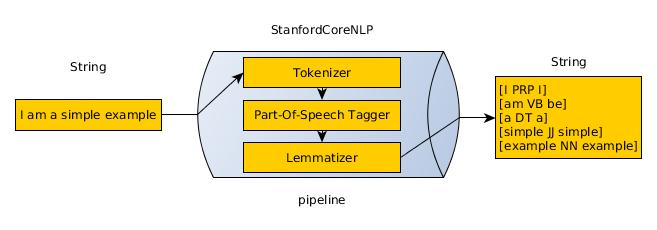
\includegraphics[width=\textwidth]{images/coreNLP.jpg}
                \caption{Trois traitements ont été assignés au \textit{pipeline} (entité de la classe \textit{StanfordCoreNLP}) : \textit{Tokenization}, \textit{POS-Tagging} et \textit{Lemmatization}. L'objet en sortie est une chaîne de caractère présentant le résultat de chaque traitement en colonne.}
                \label{fig:coreNLP}
            \end{figure}

            \subsubsection{Premier bilan sur la bibliothèque}
                Ces traitements n'ont pas tous un intérêt pour moi dans la construction de mon classifieur. En effet, dans un premier temps, mon objectif est seulement de réutiliser la partie \textit{Stanford Classifier} de la bibliothèque pour créer un classifieur binaire permettant de classifier les signaux relatifs aux offres d'emploi et de stage (soit le tag \textit{JOB}). La classe \textit{ColumnDataClassifier} pourrait mettre d'une grande aide, mais elle exige des données dans un certain format. De plus, elle ne les gère pas certain prétraitement.\\

                Enfin, il est certain que des traitements comme la lemmatisation ou le stemming me seront utiles par la suite, lorsqu'il faudra normaliser mes données. Pouvoir utiliser le \textit{StanfordCoreNLP} en amont du \textit{Stanford Classifier} pour normaliser mes données et sélectionner les features serait l'idéal, avant de les fournir au classifieur pour construire un modèle.

        \subsection{Première mise en pratique de la bibliothèque de Stanford}
        \label{ssec:premiere_mise_en_appli}
            \subsubsection{Première application Spring}
                J'ai construis une application réalisant les actions suivantes (visible en figure \ref{fig:classif_building} et expliquée ci-après) :
            \begin{itemize}
                \item Récupérer les signaux stockés dans Mongo sous forme de liste ;
                \item Créer un ensemble de données à partir des signaux validés manuellement ;
                \item Diviser aléatoirement cet ensemble de données en deux ensembles (un pour entraîner le classifieur et un pour le tester) tout en gardant la proportion de chaque classe dans les deux ensembles ;
                \item Entraîner un classifieur binaire naïf bayésien ;
                \item Fixer les hyper-paramètres du classifier par validation croisée pendant la phase d'apprentissage ;
                \item Évaluer la qualité du classifieur construit (l'erreur de généralisation) en calculant sa précision et son rappel sur un ensemble de données de test (qui n'ont pas \og été vu \fg jusqu'à ici par le classifieur).
            \end{itemize}

            \begin{figure}[h!]
                \centering
                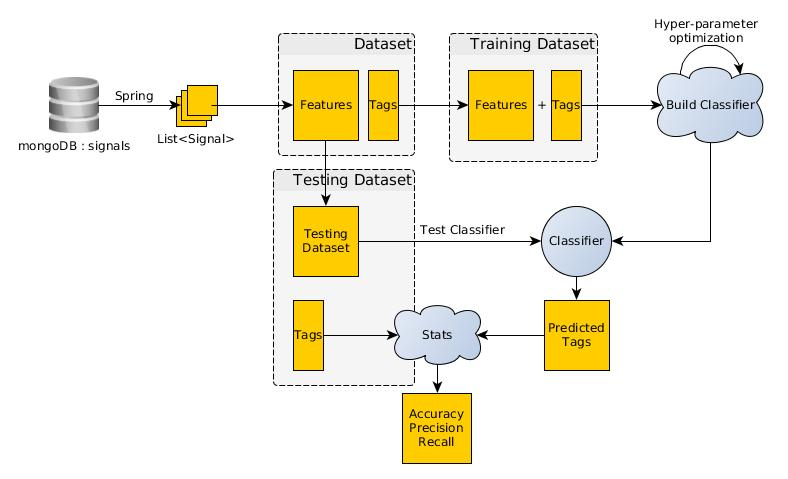
\includegraphics[width=\textwidth]{images/classifier_building.jpg}
                \caption{La construction du classifieur.}
                \label{fig:classif_building}
            \end{figure}

            \subsubsection{Le modèle de classifieur}
                La première questions, à laquelle j'ai du répondre pour pouvoir créer un premier classifieur binaire sur la classe \textit{JOB}, est la suivante : Quel type de classifieur construire ? Un SVM, une régression logistique, une modèle naïf bayésien, etc.\\
                Dans la littérature de la classification de texte, comme la détection de spam dans les emails ou l'analyse des sentiments (savoir si un texte est critique ou élogieux), il est plutôt commun de construire des classifieurs naïf bayésien avec comme caractéristiques la fréquence des mots. Ainsi, j'ai choisi de construire un tel classifieur pour catégoriser mes signaux. (C'est également ce qu'avait fait Samuel Charron en Python.)

            \subsubsection{Construction de l'ensemble de données}
                Ensuite, s'est poser la question de comment utiliser les données labellisées pour construire un ensemble de données pour l'apprentissage et la validation.\\
                Sur ce point, j'ai choisi de construire mon ensemble de données selon le modèle du sac de mots (\textit{bag of words}). Dans ce modèle, un texte (une phrase ou un document) est représenté comme un sac (\textit{bag}), un ensemble (au sens mathématique) de ses mots, sans se préoccuper de la grammaire ou de l'ordre des mots, mais en gardant la multiplicité. Ce modèle est communément utilisé en classification de document, quand la fréquence, l’occurrence des mots est utilisé comme caractéristique, attribut. Ce qui est le cas du modèle naïf bayésien. Ainsi, un signal est caractérisé par la liste des occurrences des mots formant son titre et son contenu.

            \paragraph{Exemple :}
                Voici deux signaux que l'on va modéliser à l'aide du sac de mots :
\begin{lstlisting}
K$Offre\ d'emploi\ :\ Ingénieur\ d’études\ et\ développement\ Java.$W
K$Offre\ de\ stage\ :\ Classification\ de\ signaux\ entreprises\ Java\ ou\ Python.$W
\end{lstlisting}
                À partir de ces deux signaux, une liste de mot est construite comme suit :
\begin{verbatim}
[ "Offre", "d'", "emploi", ":", "Ingénieur", "études", "et", "développement",
  "Java", ".", "de", "stage", "Classification", "signaux", "entreprises",
  "ou", "Python" ]
\end{verbatim}
                Celle-ci contient 17 mots distincts. En utilisant son index, on peut représenter chaque signal comme un vecteur de taille 17 :
\begin{lstlisting}
K$[\ 1,\ 2,\ 1,\ 1,\ 1,\ 1,\ 1,\ 1,\ 1,\ 1,\ 0,\ 0,\ 0,\ 0,\ 0,\ 0,\ 0\ ]$W
K$[\ 1,\ 0,\ 0,\ 1,\ 0,\ 0,\ 0,\ 0,\ 1,\ 1,\ 2,\ 1,\ 1,\ 1,\ 1,\ 1,\ 1\ ]$W
\end{lstlisting}
                Chaque ième composante du vecteur représente le nombre de fois que le ième mot de la liste est présent dans le signal. Par exemple, dans le premier vecteur (qui représente le premier signal), les deux premières composantes sont \og 1, 2 \fg. La première composante correspond au mot \og Offre \fg qui est le premier mot de la liste, et sa valeur est \og 1 \fg car \og Offre \fg est présent qu'une fois dans le premier signal. De la même façon, la deuxième composante correspond au mot \og d' \fg qui est le deuxième mot de la liste et sa valeur est \og 2 \fg car il est présent deux fois dans le signal. Cette représentation vectorielle ne préserve pas l'ordre des mots originel.\\

                Pour mon premier classifieur binaire naïf bayésien, l'ensemble de données a été construit suivant ce modèle, sur la base des 1426 signaux validés (présentés dans le dernier paragraphe de la partie \ref{sec:etat_bd}), en considérant seulement les 123 signaux validés \textit{JOB} comme intéressant.\\

                Enfin, aucun pré-traitement des données n'était mis en place, hors mis le fait de garder les mots dans le sac de mots final apparaissant un minimum de cinq fois. Ceci afin de supprimer les mots rares qui n'apportent pas d'informations lorsqu'on catégorise les signaux de type \textit{JOB} : les noms propres, les mots mal orthographiés ou les mots très spécifiques.

            \subsubsection{Construction du classifieur}
                Une fois le problème de la construction de mon ensemble de données résolu, j'ai construis mon classifieur binaire naïf bayésien. Pour cela, j'ai divisé mon ensemble de données en deux ensemble de données dans les proportions suivantes :
                \begin{itemize}
                    \item 75\% de l'ensemble de données pour l'ensemble d'apprentissage ;
                    \item 25\% de l'ensemble de données pour l'ensemble de test.\\
                \end{itemize}
                À noter que la méthode de la bibliothèque, permettant de diviser l'ensemble de données en deux ensembles, ne garantis pas que la proportion des classes soit conservée dans les deux ensembles résultants. De plus, l'ensemble n'est pas mélangé à chaque nouvelle construction du classifieur, il y donc un risque de sur-apprentissage. Ces deux points, je ne les avais pas pris en compte directement car cela n'était pas explicitement expliqué dans la documentation de la bibliothèque. En effet, il a fallu que je m'aperçoive que les ensembles de données étaient toujours les mêmes en phase d'apprentissage et de test pour corriger ce point. Ainsi, j'ai du lire de plus près le code source de la méthode pour ré-implémenter le bon comportement.

            \subsubsection{Optimisation des hyper-paramètres par validation croisée}
                Pour cette étape, une méthode de la bibliothèque se charge d'optimiser l'hyper-paramètre de mon classifieur naïf bayésien par validation croisée. Mon classifieur ayant été construit sur la base de l'ensemble d'apprentissage. Je l'ai donc utilisé sans aller plus loin dans les détails car la documentation n'en disait pas plus sur celui-ci et les performances en étaient bonifiées. Par la suite, j'ai repris la classe principale \textit{ColumnDataClassifier} de la bibliothèque \textit{Stanford Classifier} que j'ai refactoré. Ceci pour plusieurs raisons, et notamment pour réaliser dix plis de validation croisée lors de l'apprentissage afin d'avoir une idée de la capacité de généralisation de mon classifieur.

            \subsubsection{Évaluation de la qualité du classifieur}
                Enfin pour évaluer l'erreur de généralisation de mon classifieur, je les testais sur un ensemble de test, que le classifieur n'avait pas \og vu \fg jusque ici. J'ai calculé la précision et le rappel obtenu par la classe \textit{JOB} et par la classe \textit{USELESS} représentant le reste n'appartenant pas à \textit{JOB}. Ceux-ci sont visible en table \ref{tab:classif_perf}.
                \begin{table}[h]
                    \centering
                    \begin{tabular}{| c | c | c |}
                        \hline
                         & \textit{JOB} & \textit{USELESS} \\
                        \hline
                        Précision & 0,84 & 0,99 \\
                        Rappel & 0,91 & 0,98 \\
                        \hline
                    \end{tabular}
                    \caption{Performances du classifieurs.}
                    \label{tab:classif_perf}
                \end{table}

            \paragraph{Remarques :}
                Il est important de noter que lorsqu'on fait ce type de classification, on met l'accent sur le fait d'avoir une précision très élevée quitte à avoir un rappel un peu diminué, car quand l'un augmente l'autre diminue et vice versa.\\

                En effet, la précision mesure le nombre de fois où on a bien classifié un document. Alors que le rappel mesure le fait qu'on ait bien trouvé tout les documents d'une classe. Ainsi, on préfère se tromper très rarement dans notre classification (précision élevée) quitte à rater des signaux que l'on jugerait inutile alors que ça n'était pas le cas (rappel moyen). Ce qui est logique : on préfère qu'un utilisateur voit moins de signaux correctement classifié plutôt qu'il voit beaucoup de signaux plus ou moins correctement classifié.

            \subsubsection{Premier bilan}
                Le classifieur construit est prometteur mais il ne s'agit que d'un classifieur binaire. La généralisation à plusieurs classes, va amener à faire de nouveau choix :\\
                Faut-il adopter une stratégie de type :
                \begin{itemize}
                    \item One versus all ;
                    \item One versus One.
                \end{itemize}
                D'autres questions peuvent être soulevées comme :\\
                Est-ce que le modèle naïf bayésien va bien se généraliser en multi-classe ?\\
                Un prétraitement global n'est-il pas nécessaire ?\\
                Un prétraitement spécifique à chaque classe n'est-il pas nécessaire ?\\

        \subsection{Amélioration de ma première application et prétraitement}
            La démarche de construction du classifieur présentée dans la partie précédente (\ref{ssec:premiere_mise_en_appli}) reste la même. J'ai réutilisé (refactor) la classe \textit{ColumnDataClassifier}, afin qu'elle puisse prendre en entrée mes données provenant de Mongo et qu'elle puisse réaliser des prétraitements dessus avant de construire l'ensemble de données à partir duquel le classifieur est construit. Dans l'idéal, j'aurais aimé pouvoir réaliser les prétraitements avec le \textit{Stanford CoreNLP} mais il ne gère pas bien le français et il est très gourmand en mémoire.
            \subsubsection{Agrandissement de mon ensemble de signaux validés}
                Avant de pouvoir passer à un classifieur multi-classe, il fallait que mon ensemble de signaux validés grandissent. En effet, celui-ci souffre d'un fort déséquilibre entre les classes : il y a beaucoup plus de signaux inintéressants qu'intéressants. Je n'avais donc pas assez d'exemples de signaux intéressants pour pouvoir considérer les éventuelles prédictions d'un classifieur construit sur la base de ces données comme correctes. Il a donc été nécessaire d'en valider d'autres manuellement.

                \paragraph{Le QA ou Quality Assessment :}
                    L'objectif du QA est de demander la contribution d'un maximum de personnes sur une tâche de validation manuelle pénible.\\
                    Durant mon stage, j'ai organisé plusieurs QA pour approfondir l'ensemble des signaux d’apprentissage et de test.

                \paragraph{Proportion de signaux intéressants :}
                    La quantité de signaux n'ayant pas d'intérêt est énorme (plus de 80\% sur environ 300.000). De ce fait, une pré-sélection des signaux à valider est nécessaire. Pour cela, j'ai réutilisé le premier classifieur implémenté en Python de Samuel Charron, construit sur la base des 1426 signaux. Ce classifieur a permis de classifier des signaux non validés. Ce sont ces signaux classifiés par le classifieur Python qui ont été sélectionnés pour être validés manuellement. Notamment ceux appartenant potentiellement aux catégories EVENT, JOB et PRODUCT.\\
                    Pour ceux appartenant aux catégories MONEY et PEOPLE, ils ont été sélectionnés pour être validés à l'aide d'expressions rationnelles pour faire ressortir des termes tels que \og levée de fonds \fg, \og chiffre d'affaire \fg, \og nommer \fg, \og nomination \fg, etc.\\
                    De cette manière 2574 nouveaux signaux ont été validés manuellement. J'ai conscience que ce type de méthodes biaise la dispersion des classes de signaux intéressantes par rapport à celle sans intérêt, mais autrement il mettait impossible d'obtenir plus d'exemple.\\

                    Au 27.07.2015, il y avait donc 4000 signaux validés manuellement par un humain :
                    \begin{itemize}
                        \item 488 catégorisés EVENT soit 12,2\%
                        \item 258 catégorisés JOB soit 6,4\%
                        \item 118 catégorisés MONEY soit 3\%
                        \item 83 catégorisés PRODUCT soit 2,1\%
                        \item 49 catégorisés PEOPLE soit 1,3\%
                        \item 3004 validés mais considérés comme inintéressant soit 75\%
                    \end{itemize}

            \subsubsection{Le passage au multi-classe}
                Pour le passage au multi-classe, la bibliothèque de Stanford ne propose pas de stratégie \textit{One vs All} ou \textit{One vs One}. Je ne sais donc pas laquelle des deux est choisie. En ce qui est du modèle de classifieur, deux options s'offraient à moi :
                \begin{itemize}
                    \item Un modèle génératif et notamment un classifieur naïf bayésien ;
                    \item Un modèle discriminatif et notamment un classifieur qui maximise l'entropie.
                \end{itemize}
                Le modèle génératif maximise la vraisemblance de la probabilité jointe $P(classe, donnée)$ alors que le modèle discriminatif maximise la vraisemblance de la probabilité conditionnelle $P(classe | donnée)$. Jusque là, j'avais opté pour le modèle bayésien car c'est ce qui ressortait le plus souvent dans la littérature. J'ai donc repris mon application précédente et j'ai construit un classifieur naïf bayésien multinomial sur la base de mes 4000 signaux taggés, en employant la même méthode de construction de mon ensemble de données. Les performances obtenues (visibles en table \ref{tab:classif_perf2}) avaient grandement baissées (la classe \textit{PRODUCT} n'y figure pas car elle n'était pas suffisament représentée).
                \begin{table}[h]
                    \centering
                    \begin{tabular}{| c | c | c | c | c | c |}
                        \hline
                         & \textit{JOB} & \textit{EVENT} & \textit{PEOPLE} & \textit{MONEY} \\
                        \hline
                        Précision & 0,63 & 0,51 & 0,46 & 0,44 \\
                        Rappel & 0,91 & 0,88 & 0,63 & 0,87 \\
                        \hline
                    \end{tabular}
                    \caption{Performances du classifieur naïf bayésien multinomial.}
                    \label{tab:classif_perf2}
                \end{table}

            \subsubsection{Le modèle discriminatif maximisant l'entropie}
                Par curiosité, j'ai changé le modèle pour le modèle maximisant l'entropie car je ne connaissais pas et je voulais voir ce que ça donnerait. À ma grande surprise, le modèle discriminatif maximisant l'entropie obtint de bien meilleures performances que le modèle bayésien dans les mêmes conditions (construction de l'ensemble de données identique, prétraitements identiques, etc). Les performances sont visibles en table \ref{tab:classif_perf3}.
                \begin{table}[h]
                    \centering
                    \begin{tabular}{| c | c | c | c | c | c |}
                        \hline
                         & \textit{JOB} & \textit{EVENT} & \textit{PEOPLE} & \textit{MONEY} \\
                        \hline
                        Précision & 0,96 & 0,82 & 0,73 & 0,81 \\
                        Rappel & 0,73 & 0,60 & 0,50 & 0,49 \\
                        \hline
                    \end{tabular}
                    \caption{Performances du classifieur maximisant l'entropie.}
                    \label{tab:classif_perf3}
                \end{table}

                \paragraph{La régression logistique binomiale :}
                    Elle consiste à prédire une valeur parmi deux valeurs possibles (vrai ou faux), telle que :\\
                    $logit(\ p(x=vrai)\ )\ =\ une\ combinaison\ linéaire\ d'un\ vecteur\ de\ poids\ et\ d'un\ vecteur\ de\ traits$ ;\\
                    Cela correspond à une classification binaire qui maximise le log de vraisemblance

                \paragraph{Le \textit{MaxEnt} ou \textit{Maximum Entropy} :}
                    Les modèles \textit{maximum entropy} sont aussi connu sous le noms de \textit{softmax classifiers} et sont équivalent aux modèles de régression logistique multi-classe (avec des paramètres différents). Il s'agit de la généralisation de la régression logistique au cas multinomial. Dans ce cas, maximiser la vraisemblance revient à maximiser l'entropie. Il s'agit ni plus ni moins que du passage du cas binaire au cas N classes.\\
                    Ce type de modèle est avantageux dans le cas où les données sont \textit{sparse}. Ce qui est mon, c'est pourquoi les résultats sont meilleurs qu'avec le modèle bayésien.

            \subsubsection{Les cours de l'université de Stanford}
                Les cours de l’université de Stanford concernant le \textit{Natural Language Processing}, accessibles librement sur Internet, m'ont permis de découvrir de nombreux concepts dans ce domaine (notamment le modèle \textit{maximum entropy}). Ces cours proviennent du livre \textit{Introduction to Information Retrieval}\autocite{ir_web}.\\

                En parallèle, j'ai visionné sur coursera les vidéos que cette même université avait diffusé suite à un MOOC sur le \textit{Natural Language Processing}. Grâce à ces cours, j'ai pris conscience de toute l'importance de bien choisir son modèle de classifieur. De plus, j'ai également compris tout l'intérêt du travail de prétraitement, permettant de normaliser et formater les données textuelles afin d'augmenter les performances et la capacité de généralisation du classifieur.\\

                Durant ma formation au \textit{Natural Language Processing}, j'ai également lu les livres \textit{Natural Language Processing with Python}\autocite{nlp_p} et \textit{Python 3 Text Processing with NLTK 3 Cookbook}\autocite{nltk} , ainsi que les pages internets \textit{Introduction to Information Retrieval}\autocite{ir_web}.

            \subsubsection{Les travaux de prétraitement global}
            \label{ssubsec:travaux_globaux}
                Les traitements expliqués ci-après sont réalisés dans la construction de l'application, en amont de la construction de l'ensemble de donnée selon le modèle du sac de mot.

                \paragraph{La segmentation ou tokenisation :}
                    La tokenisation consiste à découper une phrase en token, dans l'idéal représentant des mots. Une des difficultés de cette tâche est d'être spécifique à chaque langue. Les difficultés principales sont surtout liées aux contractions. Il est nécessaire de s'attarder sur cette phase de la normalisation pour minimiser la perte sémantique, car beaucoup de traitement s'appuie sur la tokenisation. Dans mon application, j'ai utilisé le \textit{PTB Tokenizer} disponible dans \textit{Stanford Classifier}.

                    \paragraph{Exemple :}
                    Entrée : \og Je n'ai pas d'argent. En as-tu ? \fg\\
                    Sorties possibles :
                    \begin{itemize}
                        \item ["Je", "n", "ai", "pas", "d", "argent", "En", "as", "tu"]
                        \item ["Je", "n", "'", "ai", "pas", "d", "'", "argent", ".", "En", "as", "-", "tu", "?"]
                        \item ["Je", "n'", "ai", "pas", "d'", "argent", ".", "En", "as", "-", "tu", "?"]
                    \end{itemize}
                    Le résultat du \textit{PTB Tokenizer} dans l'exemple précédant est le premier.

                \paragraph{La casse, l'accentuation et la ponctuation :}
                    Pour normaliser les mots, une manière simple consiste à réduire la casse de tout les mots. Ainsi, on réduit notre ensemble de mot et dans une norme de casse. Cela est très facile à effectuer mais cela a quand même quelques défauts :
                    \begin{itemize}
                        \item Les noms propres perdent leur différences par rapport aux noms communs ;
                        \item Les noms d'organisation (comme l'OTAN) perdent leur sens en minuscule.
                    \end{itemize}
                    Une manière supplémentaire de normaliser est de supprimer les inflexions (accents). Cela n'est pas compliqué à mettre en place mais fait perdre encore une fois de l'information au texte.\\
                    Enfin, supprimer la ponctuation est aussi une manière de normaliser car celle-ci apporte très peu d'information (pour ne pas dire pas). Encore une fois, c'est simple à réaliser mais certain mot perde leur sens.
                    \begin{itemize}
                        \item Les mots composés comportant des tirets perdent leur sens (exemple : \og après-midi \fg);
                        \item Les mots composés comportant des apostrophes perdent leur sens (exemple : \og aujourd'hui \fg) ;
                        \item Les acronymes comportant des points de séparation perdent leur sens (exemple : \og U.S.A. \fg)
                    \end{itemize}

                \paragraph{Les stopwords :}
                    Les stopwords sont les mots d'une phrase inutiles à la compréhension de celle-ci. Ils ne portent pas d'information et sont présents dans n'importe quels documents textuels. Les supprimer permet donc de réduire le nombre de feature à notre ensemble de mot (le sac de mot). Une liste de stopwords contient majoritairement des pronoms, des prépositions et des déterminants comme : \og a \fg, \og au \fg, \og ce \fg, \og de \fg, \og le \fg, \og mon \fg, etc.

                \paragraph{La recherche morphologique :}
                    Enfin, les deux derniers moyens permettant de normaliser du texte sont la lemmatisation et le stemming. Ces deux traitements ont pour objectif de faire baisser le nombre de forme infléchie. Une forme infléchie est appelé un lexème en morphologie. Il faut savoir qu'un lexème est composé de différentes types de morphèmes : les stems et les affixes. Voici leur définition à l'aide d'un exemple :\\
                    Le lexème \og chanteurs \fg est composé de trois morphèmes : \og chant \fg, \og eur \fg et \og s \fg. Parmi ces trois morphèmes, un est un stem \og chant \fg et les deux autres des affixes \og eur \fg et \og s \fg.


                \paragraph{Le stemming :}
                    L'objectif du stemming est de diminuer les lexèmes en les réduisant à leur stems : \og chanteurs \fg, \og chanteuse \fg transformés en \og chant \fg.\\
                    Un des désavantage du stemming est que les stems ne sont pas toujours des lemmes, c'est à dire la forme canonique d'un lexème (son entrée dans le dictionnaire), et donc pas un mot.\\
                    Exemple : le stem de \og chercheur \fg est \og cherch \fg (n'est pas un mot).

                \paragraph{La lemmatisation :}
                    L'objectif de la lemmatisation est le même que celui du stemming à savoir diminuer le nombre de formes infléchies, de lexèmes. Pour cela, la lemmatisation consiste à réduire un lexème en lemme, la forme canonique de ce lexème. Le lemme d'un verbe correspond au verbe à l'infinitif, le lemme d'un nom commun est ce nom commun au masculin singulier, etc. Les lemmes correspondent aux entrées dans le dictionnaires de tout les lexèmes.\\

                \paragraph{Exemple :}
                    Les lemmes de la phrase \og Ils chantent leurs chansons préférées.\fg sont :\\
                     \og Il chanter leur chanson préférer. \fg

                \paragraph{Remarques :}
                    Étant donné que le stemming nous fait perdre plus d'information sur nos features que la lemmatisation, j'ai choisi d'appliquer cette dernière. De plus, avec le stemming on ne manipule plus des mots mais leur stem.\\
                    La bibliothèque de Stanford ne propose pas de Lemmatizer pour la langue française. De ce fait, j'ai utilisé une bibliothèque externe de Ahmet Aker\footnote{http://staffwww.dcs.shef.ac.uk/people/A.Aker/activityNLPProjects.html} que j'ai rajouté dans le projet Spring grâce à Maven en ajoutant une dépendance.

                \paragraph{Bilan sur les prétraitements :}
                    Ceux-ci permettent de normaliser le texte et de réduire le nombre de feature présent dans le sac de mot. Il est important de réduire la disparité des features pour pouvoir calculer leur fréquence par la suite. Un parallèle pourrait être fait avec le fait de compresser des données numériques par ACP avec la lemmatisation par exemple. Il est très important de bien préparer les données afin d'obtenir les meilleures performances possibles par la suite.

            \subsubsection{Les travaux de prétraitement spécifique}
                En plus, des traitements présentés précédemment, il est possible de traiter nos données plus spécifiquement par classe, afin d'augmenter les performances du classifieur par la suite.\\
                Pour cette tâche, il faut d'avantage s'attarder sur le fond des données de chaque classe, et essayer de voir si de l'information intéressante aurait pu être détruite par les traitement précédents.

                \paragraph{Les signaux issus de Twitter :}
                    Les signaux twitter comportent souvent des références \og @pseudo \fg et des mentions comme \og \#job \fg. Les références n'apportent pas d'information dans la majorité des cas. Les supprimer permettrait d’éliminer du bruit dans les features. Quant aux mentions comme \og \#job \fg, celles-ci portent de l'information et dans un processus de normalisation, il serait bien de garder le mot suivant le dièse (\#).

                \paragraph{Les emails et les URLs}
                    À l'image des pseudonymes Twitter, les emails et les URLs (présent dans certain signaux) ne portent aucune information et ne sont pas bien tokenisés à cause de leur formes. Ainsi, il serait bien de les supprimer en amont de la tokenisation.

                \paragraph{Les signaux de la classe \textit {JOB} :}
                    Souvent dans les offres d'emploi ou de stage, la mention \og H/F \fg signifiant \og homme ou femme \fg est présente. Cependant, lors de la tokenisation, ce genre de feature est détruit du fait qu'il contient le caractère de ponctuation slash (/). Ainsi, il serait intéressant de pouvoir les détecter avant la tokenisation et de les remplacer par une chaîne de caractère qui ne serait pas détruit par la tokenisation comme le terme \og hommeoufemme \fg.

                \paragraph{Les signaux de la classe \textit{MONEY}}
                    Une caractéristique des signaux de cette classe est que, souvent lorsque ces signaux parlent d'une levée de fonds, une somme est annoncée avec une devise. Exemple : \og L'INSA a levée 5 k€ pour construire un amphithéâtre \fg.\\
                    Il serait donc intéressant de conserver l'unité et le symbole de la devise suivant le montant qui est caractéristique de ce type de signal (k€, m€, etc).

                \paragraph{Mise en place de ces traitements et bilan :}
                    J'ai implémenté ces traitements assez facilement à l'aide d'expressions rationnelles. Ce travail d'inspection du contenu des signaux est important car c'est là que l'on détecte des informations caractéristiques.

            \subsubsection{Performances obtenues par mon application avec les prétraitements}
                \paragraph{Le problème des FP (faux positifs) :}
                    Les signaux qui peuvent avoir potentiellement plusieurs labels engendrent une quantité non négligeable de faux positifs, comme par exemple :
                    \begin{itemize}
                        \item Signal : "Venez découvrir nos nouveautés produits du 20 au 22 Mai 2014 au salon SEPEM, Hall 4 - Stand F13 http://t.co/vS7gT2x4yp \#marquagepermanent" Label : PRODUCT ou EVENT
                        \item Signal : "Nous embauchons! Étudiants de HEC Paris, nous sommes aujourd'hui au \#CarrefoursHEC. Venez découvrir nos offres d'emploi dans les domaines du \#digital \#data \#marketing" Label : JOB ou EVENT
                    \end{itemize}
                    Une solution potentielle serait d'autoriser le classifieur à attribuer plusieurs label. C'est ce qu'avait fait Samuel Charron en Python mais les résultats n'étaient pas suffisant.

                \paragraph{Le problème des FN (faux négatifs) :}
                    Les signaux ne sont pas toujours très succins et précis. De ce fait, parfois en plus d'un contenu intéressant le signal peut contenir du bruit, ce qui engendre une quantité non négligeable de faux négatifs. Ce qui baisse les rappels. Exemple :
                    \begin{itemize}
                        \item Signal : "Dans le cadre de son développement, EXCELIUM a fait l'acquisition du fonds de commerce de la société lyonnaise SES Vidéo, spécialisée dans l'installation de systèmes vidéo et d'alarme." Label : Aucun alors que c'est MONEY
                        \item Signal : "A l'occasion de la fête de la gastronomie, nous vous invitons à visiter notre nouveau laboratoire à Téteghem samedi 27 septembre de 10 h à 18h. Visite, dégustation et chèques cadeaux offerts pour toute commande passée sur le site cette semaine !" Label : aucun alors que c'est EVENT
                    \end{itemize}

                \paragraph{Performances du classifieur sur l'ensemble des 4000 signaux validés :}
                    Les performances présentés en table \ref{tab:classif_perf4} ont été obtenues en construisant le classifieur en suivant les étapes décrites dans la partie \ref{ssec:premiere_mise_en_appli}.
                    \begin{table}[t]
                        \centering
                        \begin{tabular}{| c | c | c | c | c | c |}
                            \hline
                             & \textit{JOB} & \textit{EVENT} & \textit{PEOPLE} & \textit{MONEY} \\
                            \hline
                            Précision & 0,96 & 0,82 & 0,94 & 0,81 \\
                            Rappel & 0,81 & 0,63 & 0,60 & 0,60 \\
                            \hline
                        \end{tabular}
                        \caption{Performances du classifieur maximisant l'entropie.}
                        \label{tab:classif_perf4}
                    \end{table}

                \paragraph{Performances du classifieur sur un ensemble de données non vus (obtenus grâce à un QA) :}
                    341 718 signaux ont été tagué automatiquement par le classifieur entraîné sur 4000 signaux validés.
                    (Certaines sources de signaux sont blacklistées et leurs signaux émis ne sont donc pas taguées par le classifieur : Les entreprises d'interim, les chasseurs de tête, les e-commerçants, etc). Parmi tout ces signaux, 388 ont été validé manuellement lors d'un QA. Ces signaux validés ont été sélectionnés aléatoirement parmi les 341 718 signaux tagués par le classifieur. Voici les résultats :
                    \begin{table}[t]
                        \centering
                        \begin{tabular}{| c | c | c | c | c | c | c |}
                            \hline
                             & \textit{JOB} & \textit{EVENT} & \textit{PEOPLE} & \textit{PRODUCT} & \textit{MONEY} \\
                            \hline
                            Précision & 0,98 & 0,70 & 0,83 & 0,56 & 0,51 \\
                            Rappel & 0,92 & 0,80 & 0,97 & 0,75 & 0,95 \\
                            \hline
                        \end{tabular}
                        \caption{Performances du classifieur sur des données non validées.}
                        \label{tab:classif_perf4}
                    \end{table}

                Malgré tout, grâce à tout ces prétraitements, mon classifieur a obtenu de meilleures performances, jugées suffisantes par mon maître de stage Samuel Charron pour que je puisse passer à l'implémentation en Python. Les classes \textit{PRODUCT} et \textit{MONEY} manque d'exemple représentatif, d'où leur mauvais résultat. Un QA supplémentaire sur ces classes leur permettrait de se bonifier.

\chapter{Conclusion}
Ce stage a été une expérience très enrichissante tant sur le plan humain et relationnel, que sur le plan technique. Je souhaitais absolument découvrir l'univers de la start-up et c'est chose fait grâce à Data Publica et ses équipes.\\

Sur le plan humain, j'ai eu la chance de rencontrer des personnes extrêmement sympathiques et compétentes, mais aussi ouvertes à la discussion et toujours disponible. L'équipe de Data Publica m'aura toujours bien encadré. Que ce soit Samuel Charron (et Christian Frisch) pendant la première partie stage ou Clément Chastagnol (et Guillaume Lebourgeois) en deuxième partie, j'aurais constamment eu quelqu'un à mon écoute. En effet, lorsque je rencontrais une difficulté, j'avais, à chaque moment, quelqu'un de disponible à \og déranger \fg pour mettre à l'épreuve son expérience ou ses connaissances.\\

Un excellent stage sur le plan relationnel aussi. En effet, tout le monde m'a accordé du temps à mon arrivée pour se présenter, et me dire leurs tâches et responsabilités chez Data Publica. De plus, partager des déjeuners et des pots conviviales a permis de renforcer et aussi de créer de premiers liens avec les collègues.\\

J'ai également beaucoup aimé cet esprit de partage et ces discussions ouvertes, lors des réunions des équipes pour différents points.\\

Sur le plan technique, j'ai énormément progressé dans le domaine du \textit{machine learning} et énormément appris dans le domaine du \textit{text mining} que je ne connaissais pas. Tous ces concepts de normalisation de textes, le langage Python et ses modules disponibles (scikit-learn, numpy, nltk, etc). J'ai découvers une facette de la \textit{data science} que j'ignorais et qui m'a beaucoup plue.\\

Ce stage aura donc été très riche, techniquement parlant, par la découverte de domaines inconnus et passionnants, mais aussi humainement parlant, par la rencontre de personne formidable et poussant constamment à la réussite et au dépassement de soi.



\chapter{Résumé}
\input{parties/05-Resume.tex}

% Bibliographie
%\bibliographystyle{plain}
\printbibliography

% Annexes
\clearpage
\appendix
\chapter{Annexes}
\section{Les métriques de mesure de la qualité d'une classification}
    \subsection{Terminologies}
        Pour une classe donnée, voici la signification de ces terminologies :
        \begin{itemize}
            \item $\highlight[green]{TP}$ : True positive, bonne assignation à la classe ;
            \item $\highlight[green]{TN}$ : True negative, bon rejet de la classe ;
            \item $\highlight[red]{FP}$ : False positive, mauvaise assignation à la classe ;
            \item $\highlight[red]{FN}$ : False negative, mauvais rejet de la classe.
        \end{itemize}

    \subsection{La précision}
    \label{annexe:precision}
        Pour une classe donnée, la précision est le nombre de documents correctement assignés à cette classe rapporté au nombre de documents total assignés à cette classe par le classifieur.\\
        $Précision\ =\ \frac{TP}{TP+FP}$


    \subsection{Le rappel}
    \label{annexe:rappel}
        Pour une classe donnée, le rappel est défini par le nombre de documents correctement assignés à cette classe au regard du nombre total de documents appartenant réellement à cette classe.\\
        Le rappel mesure le fait que le classifieur ait trouvé tous les documents d'une classe.\\
        $Rappel\ =\ \frac{TP}{TP+FN}$

\section{Le QA ou Quality Assessment}
\label{annexe:qa}
    L'objectif du QA est de demander la contribution d'un maximum de personnes sur une tâche de validation manuelle pénible.\\

\section{Modèle de classifieur}
    Les points d'explication qui suivent, sont en partie tirés de Wikipédia\autocite{wiki_discri_gene}.
    \subsection{Le modèle génératif}
    \label{annexe:generatif}
        Le modèle génératif consiste à modéliser les probabilités conditionnelles soit $P(donnée | classe)$. Voici quelques exemples d'algorithmes de ce type :
        \begin{itemize}
            \item Classifieur naïf bayésien implique une distribution de probabilité conditionnelle de type binomiale (ou multinomiale) ;
            \item Analyse discriminante linéaire (LDA). Elle implique l'existence d'un modèle discriminant basé sur une distribution de probabilité de type Gaussienne.
        \end{itemize}
        Le modèle génératif maximise la vraisemblance de la probabilité jointe $P(classe, donnée)$.

    \subsection{Le modèle discriminant}
    \label{annexe:discriminatif}
        Le modèle discriminant cherche à maximiser la qualité de la classification. Une fonction de coût va réaliser l'adaptation du modèle de classification (en minimisant les erreurs). Voici quelques exemples d'algorithmes de ce type :
        \begin{itemize}
            \item Régression logistique, maximisation de la vraisemblance en considérant que les données suivent un modèle binomial ;
            \item Support Vectort Machine (SVM), maximisation de la marge entre l'hyperplan séparant les données.
        \end{itemize}
        Le modèle discriminatif maximise la vraisemblance de la probabilité conditionnelle $P(classe | donnée)$.

\section{Les transducteurs}
\label{annexe:transducteurs}
    Définition tirée de Wikipédia\autocite{wiki_trans}.\\

    En informatique théorique, en linguistique, et en particulier en théorie des automates, un transducteur fini (appelé aussi transducteur à états finis par une traduction maladroite de l'anglais finite state transducer) est un automate fini avec sorties. C'est une extension des automates finis. Ils opèrent en effet sur les mots sur un alphabet d'entrée et, au lieu de simplement accepter ou refuser le mot, ils le transforment, de manière parfois non déterministe, en un ou plusieurs mots sur un alphabet de sortie. Ceci permet des transformations de langages, et aussi des utilisations variées telles que notamment l'analyse syntaxique des langages de programmation, et l'analyse morphologique ou l'analyse phonologique en linguistique.\\

    D'autres explications détaillées sont disponibles \href{http://sixty-north.com/blog/deriving-transducers-from-first-pr}{ici}.


% pageQuatriemeCouverture
% #1 : Direction
% #2 : telephone
% #3 : e-mail
% #4 : Resume Haut
% #5 : Resume Bas
\pageQuatriemeCouverture{Département ASI}{02 32 95 97 79}{asi@insa-rouen.fr}{Ce stage obligatoire s'effectue en fin de quatrième année. Au cours de ce stage l'étudiant devra mettre en pratique les connaissances acquises au cours de sa formation et devra approfondir son savoir-faire au sein de l'entreprise. Il faudra qu'à  la fin de son stage l'étudiant réalise un rapport écrit. La validation du stage dépend de la qualité du travail réalisé, du rapport et de la fiche d'évaluation du tuteur industriel.\\
Ce stage a eu lieu chez Data Publica, un des précurseurs de l'open data en France. Data Publica est une jeune start-up (fondée en juillet 2011) spécialisée dans les données entreprises, l'open data, le big data et la dataviz. Data Publica emploie quatorze personnes très dynamiques et compétentes. Data Publica développe C-Radar, un produit de vente prédictive construit sur une base de référence des entreprises françaises regroupant informations administratives, financières, web, réseaux sociaux et media. C-Radar est un concentré de technologies du big data (crawling, scraping ou encore machine learning).\\
Ma mission, chez Data Publica, est de construire une chaîne de traitement automatique, un plugin Python, récupérant une liste de documents textuels en entrée et fournissant, en sortie, une liste de ces documents labellisés selon leur catégorie d'intérêt (offre d'emploi, participation à des événements, nomination de personnel, levée de fond, etc).\\
Les tâches qui en découlent sont directement liées au \textit{Text Mining} et au \textit{Natural Language Processing} (aussi à l'\textit{Information Retrieval}) dans la découverte d'informations dans le contenu des documents. Des compétences en \textit{Machine Learning} sont également requises.\\
Ce stage s'est conclue de belle manière, puisque le plugin Python est fonctionnel et capable de classifier de tels documents.}{This internship is obligatory and carried out at the end of the fourth year. During this internship, the student shall put into practice the knowledge acquired during his training and shall get better skills whithin the company. At the end of the intership, the student must write a report. The internship validation is depending on the quality of the work, the report and the evaluation sheet of the industrial tutor.\\
This internship took place at Data Publica, an open data pioneer in France. Data Publica is a young start-up (founded in July 2011) specialized in business data, open data, big data and DataViz. Data Publica employs 14 dynamic and competent people. Data Publica is developing C-Radar, a predictive selling product built on French enterprises informations, like administrative, financial, web, social networks and media. C-Radar is made of big data technologies (crawling, scraping or machine learning).\\
My mission at Data Publica, is to build an automatic processing chain, a Python plugin, which giving a list of textual records as input, get back a list of tagged documents according to their interest subject (job offer, event participation, staff nomination, fundraising, etc).\\
The directed tasks linked to the detection of information in the records are Text Mining and Natural Language Processing (also Information Retrieval). Skills in Machine Learning are also required.\\
This internship completed well, because the Python plugin is running and able to classify records.}



\end{document}
